\documentclass[12pt]{report}
\usepackage[a4paper]{geometry}
\usepackage[colorlinks=false, pdfborder={0 0 0}]{hyperref}
\usepackage[utf8]{inputenc}
%\usepackage{amsmath}
%\usepackage{booktabs}
%\usepackage{cleveref}
\usepackage{graphicx}
%\usepackage{microtype}
%\usepackage{siunitx}
%\usepackage{xgreek}
\graphicspath{ {images/} }

\RequirePackage[l2tabu, orthodox]{nag}


\title{
	{Thesis Title}\\
	{\large Aristotle University of Thessaloniki}\\
	{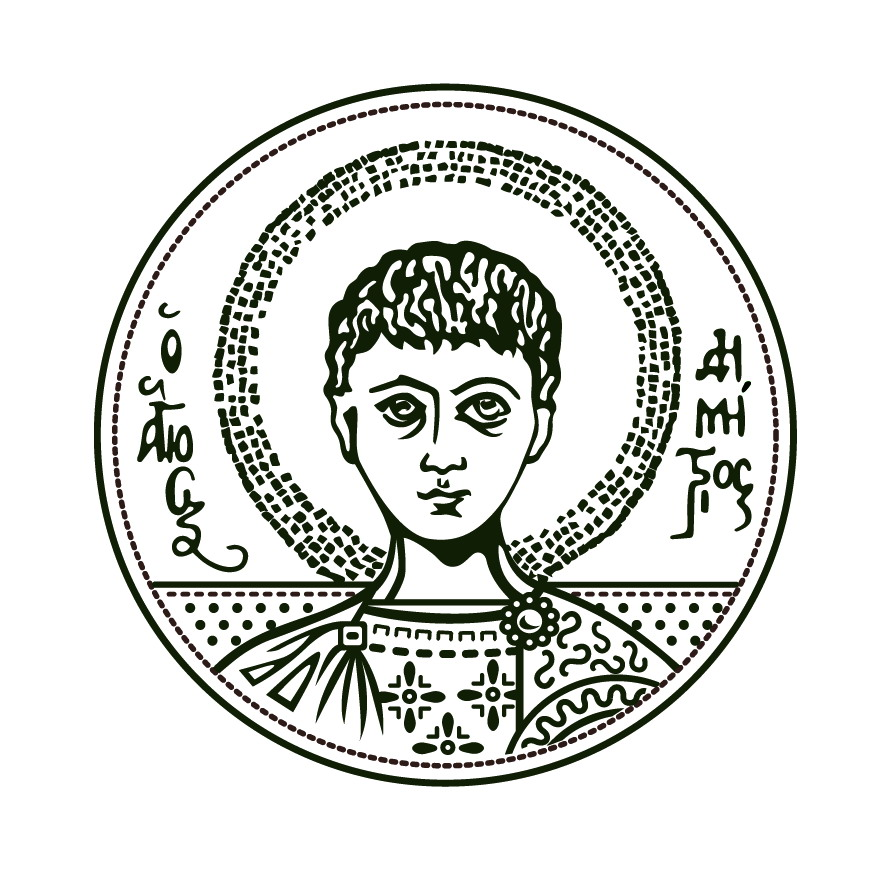
\includegraphics{auth-logo.jpg}}
}
\author{Orfeas Antoniou}
\date{Day Month Year}
\begin{document}

\maketitle
\chapter*{Abstract}
Lorem Ipsum is simply dummy text of the printing and typesetting industry. Lorem Ipsum has been the industry's standard dummy text ever since the 1500s, when an unknown printer took a galley of type and scrambled it to make a type specimen book. It has survived not only five centuries, but also the leap into electronic typesetting, remaining essentially unchanged. It was popularised in the 1960s with the release of Letraset sheets containing Lorem Ipsum passages, and more recently with desktop publishing software like Aldus PageMaker including versions of Lorem Ipsum.

\chapter*{Dedication}
To mum and dad

\chapter*{Declaration}
I declare that..

\chapter*{Acknowledgments}
I want to thank...

\tableofcontents

\chapter{Introduction}
Lorem ipsum dolor sit amet, consectetur adipiscing elit. Pellentesque dapibus nisi sit amet massa rutrum bibendum. Suspendisse pellentesque, arcu non interdum placerat, metus ex ullamcorper odio, ac mattis enim erat a tellus. Morbi consectetur tortor a sagittis pharetra. Donec in tempus est. In placerat, sem ac posuere suscipit, enim metus bibendum ex, in condimentum risus sapien ut est. In gravida diam sit amet sapien viverra cursus. Donec mattis ipsum vel diam luctus, in porttitor erat dapibus. Vestibulum mauris diam, cursus at consequat vel, maximus sit amet est. Suspendisse ultrices magna egestas est tempus, non imperdiet leo condimentum. Aliquam erat volutpat. Aenean vitae tincidunt massa.

Quisque sit amet dignissim magna. Cras posuere leo at posuere interdum. Curabitur a libero metus. Duis at arcu ac arcu placerat volutpat. Morbi posuere consequat ornare. Integer aliquam diam justo, vel rhoncus ex venenatis sed. Cras id euismod orci. Suspendisse potenti. Etiam at nibh vitae purus aliquet bibendum nec sed diam. Proin suscipit ullamcorper facilisis. Duis eget mattis ex, at imperdiet metus. Vestibulum imperdiet ex non massa vehicula rhoncus. Cras vehicula elit in laoreet ultricies. Mauris eget neque faucibus massa sagittis consectetur. Suspendisse enim felis, convallis nec sapien at, maximus rhoncus risus.

Mauris ac efficitur erat, et tincidunt lacus. Aenean tempor dolor lorem, a finibus lacus auctor a. Aliquam non luctus est. Sed augue purus, posuere dictum ligula at, tempus egestas eros. Cras volutpat ex nisi, eget tempor mauris efficitur at. Quisque ut aliquam turpis. Duis aliquet porttitor urna, a dignissim purus mollis eu. Donec maximus, tellus convallis ultrices malesuada, libero magna tincidunt diam, rutrum ultricies leo nulla nec ligula. Sed iaculis, mi at pellentesque venenatis, mauris elit iaculis eros, quis iaculis massa libero quis augue. Fusce nec odio libero. Duis orci metus, lacinia quis tortor eu, fringilla finibus nunc. Pellentesque et pulvinar mi.

Pellentesque tincidunt neque et ullamcorper ornare. Donec euismod mollis consectetur. Duis et tellus sed massa scelerisque dapibus ut sit amet magna. Sed efficitur turpis erat, nec cursus tellus consequat vitae. Pellentesque habitant morbi tristique senectus et netus et malesuada fames ac turpis egestas. Curabitur consequat turpis in tellus malesuada, ac iaculis nulla fermentum. Ut tincidunt ipsum libero, at mollis ante luctus at. Aenean ac tellus sit amet dolor efficitur semper et non eros. Fusce hendrerit accumsan commodo. Praesent commodo, lacus nec luctus interdum, lacus sem vehicula est, sed commodo arcu sem vel nulla.

Sed diam mauris, viverra a sem sit amet, cursus posuere nunc. Morbi vel fringilla dolor. Aliquam finibus nibh id varius placerat. Nullam velit ante, tincidunt at dolor eget, tincidunt pellentesque ipsum. Suspendisse ut finibus odio. Aliquam a magna sit amet augue pulvinar gravida et in eros. Aliquam a orci quis tortor tempor mattis vel nec magna.

Vestibulum pellentesque neque vitae nibh sodales tempor. Curabitur posuere euismod enim non blandit. Nunc ex odio, venenatis ac efficitur a, hendrerit et est. Etiam vitae porta urna. Aliquam hendrerit urna quis sem feugiat, vel pharetra lectus cursus. Maecenas purus neque, eleifend vel elit non, molestie vestibulum augue. Fusce semper mauris et pharetra bibendum. Mauris hendrerit erat sed magna consequat, at eleifend elit dictum. Proin nisi lectus, tempus at sollicitudin at, vehicula sed tortor. Praesent dapibus nunc a tortor ullamcorper auctor. Suspendisse dapibus, velit et tristique laoreet, massa libero interdum augue, non porttitor lacus metus vitae lorem. Vivamus ut placerat augue. Class aptent taciti sociosqu ad litora torquent per conubia nostra, per inceptos himenaeos. Maecenas vestibulum purus in rhoncus auctor. Fusce in sem nisl.

Vivamus et felis eget diam tincidunt commodo. Integer vel nibh sit amet nisl gravida hendrerit. Quisque dictum libero ut posuere auctor. Maecenas ut sagittis dui, vitae tempus metus. Donec vestibulum quam neque, vehicula sodales nulla hendrerit vel. Nullam dictum finibus risus, elementum euismod libero imperdiet non. Nulla id urna facilisis, sagittis orci vel, fringilla tortor. Vivamus mattis lorem quis tellus tristique tempus. Interdum et malesuada fames ac ante ipsum primis in faucibus. Suspendisse quis sapien nibh. Nullam interdum lacus et risus rhoncus molestie non id libero. Cras fermentum ligula at tortor elementum imperdiet.

Quisque tincidunt mi malesuada arcu eleifend, sit amet euismod ante lobortis. Vivamus id nisl eu mauris mollis rhoncus. Mauris ut lorem turpis. Duis suscipit lectus lorem, vel volutpat nisl molestie eget. Mauris convallis sem vitae felis convallis, sed malesuada ante rutrum. Vivamus pellentesque purus non est interdum varius. Quisque at dui et dolor fringilla commodo a feugiat nibh. Nulla non odio venenatis, vestibulum nulla sed, porta libero. In ornare rutrum orci sed porta. Duis mattis, ex eu facilisis egestas, nisl dui sollicitudin diam, ut elementum ex risus a mi.

Mauris odio libero, rutrum nec diam nec, molestie rhoncus magna. Nunc id dictum diam. Donec ut commodo nisl, et accumsan magna. Suspendisse vestibulum eget purus porttitor vestibulum. Sed sagittis, mauris ut ultricies malesuada, elit erat condimentum dui, nec cursus mauris sem a lectus. Vestibulum ante ipsum primis in faucibus orci luctus et ultrices posuere cubilia Curae; Donec vel mollis quam. Nulla facilisi. Quisque fringilla pretium nibh, at dictum lacus accumsan sed. Maecenas in ligula id sapien ultricies rhoncus eget eu odio. Duis at turpis vitae metus luctus semper. Nulla bibendum nulla nibh, vel fringilla lectus dictum et.

Suspendisse potenti. Sed sagittis tincidunt velit, nec rhoncus tortor interdum eget. Sed non tortor diam. Duis iaculis convallis lectus sit amet sodales. Mauris ante dolor, aliquam non magna eleifend, ornare tempor velit. Pellentesque molestie risus non venenatis consectetur. Integer et metus vehicula, mollis justo ultricies, finibus tellus. Nunc mauris ante, faucibus a urna sed, ultricies placerat mauris. Curabitur justo dui, elementum a congue sed, posuere vitae orci.

Vivamus eleifend sagittis viverra. Sed rutrum tincidunt augue in auctor. Suspendisse ullamcorper justo quis commodo consequat. Etiam eu nibh id massa imperdiet placerat at vel nisl. Nullam tellus metus, porttitor ut laoreet eget, rutrum et libero. Nam nisi augue, placerat ut sodales quis, vestibulum nec eros. Pellentesque ac elementum dui. Quisque varius pellentesque commodo. Nunc sit amet ornare nibh. Mauris finibus ante eget arcu cursus molestie. Mauris vestibulum, urna in egestas dignissim, massa augue pellentesque ante, nec finibus mauris quam eget arcu. Phasellus sed ex enim. Proin suscipit lorem vitae eros condimentum iaculis. Aliquam malesuada posuere augue. Quisque pellentesque mauris sed pharetra imperdiet. Vivamus eu leo sit amet tellus ornare bibendum.

Ut ut rhoncus arcu, vitae accumsan mi. Interdum et malesuada fames ac ante ipsum primis in faucibus. Morbi tristique posuere varius. Maecenas semper vulputate mollis. Curabitur consectetur viverra tortor, et consequat urna suscipit iaculis. Cras velit nibh, pulvinar ut nisi sit amet, dictum fermentum sem. Pellentesque consectetur eleifend arcu, sed sagittis velit pharetra ut. Morbi tristique ut mi vitae finibus. Integer nec lorem eu ligula egestas eleifend.

Vivamus quis consectetur magna, non feugiat ex. Nullam erat nisi, ornare vitae dignissim a, vulputate vel risus. Phasellus lobortis dui vitae tortor bibendum, vitae ornare leo accumsan. Pellentesque tincidunt accumsan arcu, vel dictum massa varius et. Cras pellentesque faucibus sapien, et vulputate dui tristique quis. Cras vulputate eleifend finibus. Ut a tortor nisl. In ut consectetur arcu.

Sed maximus lacus non sem vehicula imperdiet. Donec facilisis pharetra nulla et rhoncus. Etiam convallis id magna vel tincidunt. Vestibulum a metus nec urna pharetra bibendum. Fusce et sem a lacus rutrum euismod. Aenean mollis feugiat quam sed blandit. Suspendisse potenti. Donec consequat ex quis leo pharetra, vel sodales nibh venenatis. Phasellus elit magna, dignissim ac accumsan ac, porta in lorem.

Nam vel enim ut purus luctus rutrum at vitae ex. Proin sagittis ex sit amet leo congue, in accumsan risus ultrices. Donec sodales vel ipsum quis lobortis. Integer faucibus odio non leo tempus, rutrum auctor felis efficitur. Sed euismod nulla diam. Nam in libero commodo, laoreet neque at, pharetra mi. Fusce quam libero, euismod et purus sit amet, elementum ullamcorper erat. Curabitur vitae sem semper, rutrum dui sit amet, ultricies turpis. Duis eu pulvinar ante, sit amet molestie elit. Sed ante dolor, semper quis laoreet eu, volutpat ac arcu. Morbi tortor enim, luctus et vestibulum vitae, vulputate id risus. Fusce posuere nunc at est tincidunt congue. Donec venenatis sodales nulla, sed facilisis nulla interdum id. Pellentesque pulvinar nisi ut metus congue, sed volutpat justo vulputate.

\chapter{Chapter Two Title}
\chapter{\selectlanguage{greek}Θεωρητικό υπόβαθρο}
\begin{itemize}
\item περιγραφή πειράματος και
\item Για να καταλάβει ο κόσμος τι σημαίνει
\item Γιατί είναι χρήσιμο
\item Φωτογραφίες
\item Τι χρειάζεται να ξέρω
\item Το πείραμα
\end{itemize}

Στο κεφάλαιο αυτό παρουσιάζονται αναλυτικά οι 

\section{\selectlanguage{greek}Το \en{CERN}}

To \en{CERN}, διατηρώντας το ακρωνύμιο της αρχικής Γαλλικής ονομασίας του \en{Conseil Européen pour la Recherche Nucléaire}, είναι το μεγαλύτερο σε έκταση πειραματικό κέντρο πυρηνικών ερευνών και ειδικότερα επί της σωματιδιακής φυσικής στον κόσμο. 
Βρίσκεται δυτικά της Γενεύης, στα σύνορα Ελβετίας και Γαλλίας. 
Ιδρύθηκε το 1954 από 12 ευρωπαϊκές χώρες και σήμερα αριθμεί 20 κράτη-μέλη, μεταξύ των οποίων και η Ελλάδα, η οποία είναι και ιδρυτικό μέλος.

\begin{figure}[h]

\includegraphics[scale=0.7]{images/LogoBadge-01.png}
\centering
\caption{Το λογότυπο του \en{CERN}}
\label{CERNlogo}
\end{figure}

Η βασική λειτουργία του \en{CERN} είναι η παροχή επιταχυντών σωματιδίων και άλλων υποδομών απαραίτητων για την έρευνα στον τομέα της φυσικής υψηλών ενεργειών και ως αποτέλεσμα έχουν πραγματοποιηθεί πολυάριθμα πειράματα στο \en{CERN} μέσω διεθνών συνεργασιών.

Επίσης, το \en{CERN} αποτελεί τη γενέτειρα του Παγκόσμιου Ιστού (\en{World Wide Web}).
Στην κύρια τοποθεσία του στο \en{Meyrin} βρίσκεται μεγάλη εγκατάσταση ηλεκτρονικών υπολογιστών με ισχυρές υποδομές επεξεργασίας δεδομένων, κυρίως για την ανάλυση των πειραματικών δεδομένων. 
Λόγω της ανάγκης να καταστούν αυτές διαθέσιμες σε εξωτερικούς ερευνητές, υπήρξε ιστορικά ένας σημαντικός κόμβος δικτύου ευρείας περιοχής (\en{Wide Area Network}).

Αρκετά σημαντικά επιτεύγματα στο πεδίο της φυσικής των σωματιδίων έγιναν μέσω πειραμάτων στο \en{CERN}. Αυτά περιλαμβάνουν:
\begin{itemize}
\item 1973: Ανακάλυψη των ουδέτερων ρευμάτων στο θάλαμο φυσαλίδων \en{Gargamelle}.
\item 1983: Ανακάλυψη των μποζονίων $W$ και $Z$ στα πειράματα \en{UA1} και \en{UA2}.
\item 1995: Πρώτη δημιουργία ατόμων αντιυδρογόνου στο πείραμα \en{PS210}.
\item 1999: Ανακάλυψη της άμεσης παραβίασης \en{CP} στο πείραμα \en{NA48}.
\item 2010: Απομόνωση 38 ατόμων αντιυδρογόνου.
\item 2011: Διατήρηση αντιυδρογόνου για πάνω από 15 λεπτά.
\item 2012: Ένα μποζόνιο με μάζα περίπου \SI[per-mode = symbol]{125}{\GeV \per  \clight \squared} συνάδει με τον πολυπόθητο μποζόνιο \en{Higgs}.
\end{itemize}


\section{\selectlanguage{greek}Ο επιταχυντής \en{CLIC}}

Ο \en{CLIC -- Compact Linear Collider} -- αποτελεί μια μελέτη για ένα μελλοντικό επιταχυντή που θα φτάσει σε πρωτοφανή επίπεδα ενέργειας ηλεκτρόνια και αντισωμάτιά τους, ποζιτρόνια. 
Όταν θα έρχονται σε επαφή μέσω σύγκρουσης, θα καταστρέφουν το ένα το άλλο, απελευθερώνοντας όλη τους την ενέργεια για την παραγωγή νέων σωματιδίων.

Τα ηλεκτρόνια και τα ποζιτρόνια είναι θεμελιώδη σωματίδια και οι συγκρούσεις τους μπορούν να προσφέρουν εξαιρετικά λεπτομερείς πληροφορίες σχετικά με τους νόμους της φύσης. 
Έτσι ο \en{CLIC} θα προσφέρει σημαντικές θεμελιώδεις γνώσεις φυσικής, πέρα από αυτές που είναι διαθέσιμες από το Μεγάλο Επιταχυντή Αδρονίων (\en{Large Hadron Collider -- LHC}) ή από ένα γραμμικό επιταχυντή ηλεκτρονίων/ποζιτρονίων χαμηλότερης ενέργειας, λόγω του μοναδικού συνδυασμού πειραματικής ακρίβειας και υψηλής ενέργειας.

Σε αυτές τις υψηλές ενέργειες, τα ηλεκτρόνια και ποζιτρόνια θα έχαναν ένα τεράστιο μέρος της ενέργειάς τους επιταχυνόμενα σε έναν κυκλικό επιταχυντή σαν τον \en{LHC}. 
Έτσι, τα σωματίδια πρέπει να επιταχυνθούν σε δύο γραμμικούς επιταχυντές που αντικρίζουν ο ένας τον άλλο, έτσι ώστε οι δέσμες να συγκρούονται στον κεντρικό ανιχνευτή. 
Αυτό συνεπάγεται ότι τα σωματίδια πρέπει να αποκτήσουν την ενέργειά τους από ένα και μόνο πέρασμα τους μέσα από τις κοιλότητες επιτάχυνσης.

\begin{figure}[h]
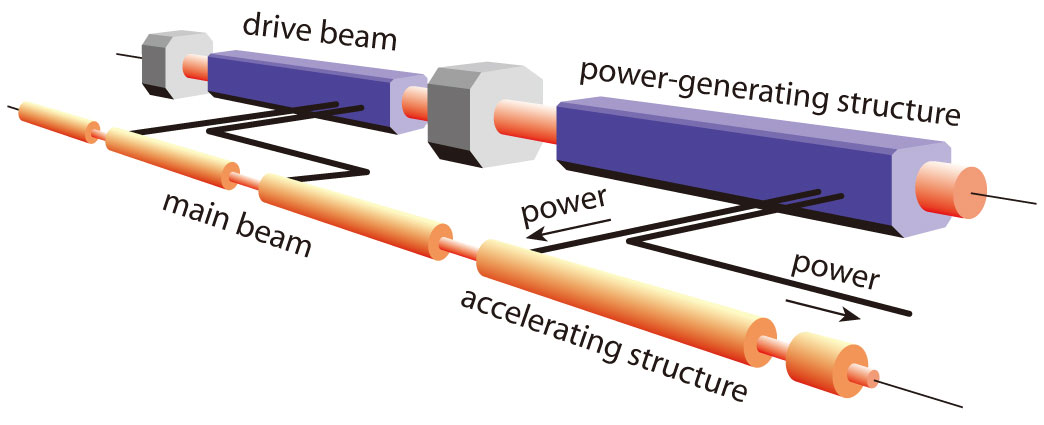
\includegraphics[width=0.5\textwidth]{images/CLIC-twobeam.jpg}
\centering
\caption{Το σύστημα δύο δεσμών του \en{CLIC}}
\label{CLICtwobeamscheme}
\end{figure}

Ο \en{CLIC} έχει σχεδιαστεί για να κατασκευαστεί σε στάδια αυξανόμενης ενέργειας για σύγκρουση: ξεκινώντας από \SI{360}{\GeV}, περίπου \SI{1.4}{\TeV}, και μέχρι την τελική ενέργεια των \SI{3}{\TeV}. 
Προκειμένου να επιτευχθεί αυτή η ενέργεια με ένα ρεαλιστικό και οικονομικά αποδοτικό τρόπο, η αύξηση της επιτάχυνσης πρέπει να είναι πολύ υψηλή.
Ο \en{CLIC} αποσκοπεί σε επιτάχυνση των \SI[per-mode = symbol]{100}{\mega \volt \per \metre}, 20 φορές υψηλότερη από αυτή του \en{LHC}.

Αυτή η δέσμη-οδηγός (drive beam) επιβραδύνεται σε ειδικές Διατάξεις Εξαγωγής και Mεταφοράς Ισχύος -- \en{Power Extraction and Transfer Structures (PETS)}, και η παραγόμενη \en{RF} ισχύς μεταφέρεται στην κύρια δέσμη. 
Αυτό οδηγεί σε μια πολύ απλή διάταξη σήραγγα χωρίς ενεργά \en{RF} μέρη (δηλ. \en{klystrons}).

\begin{figure}[h]
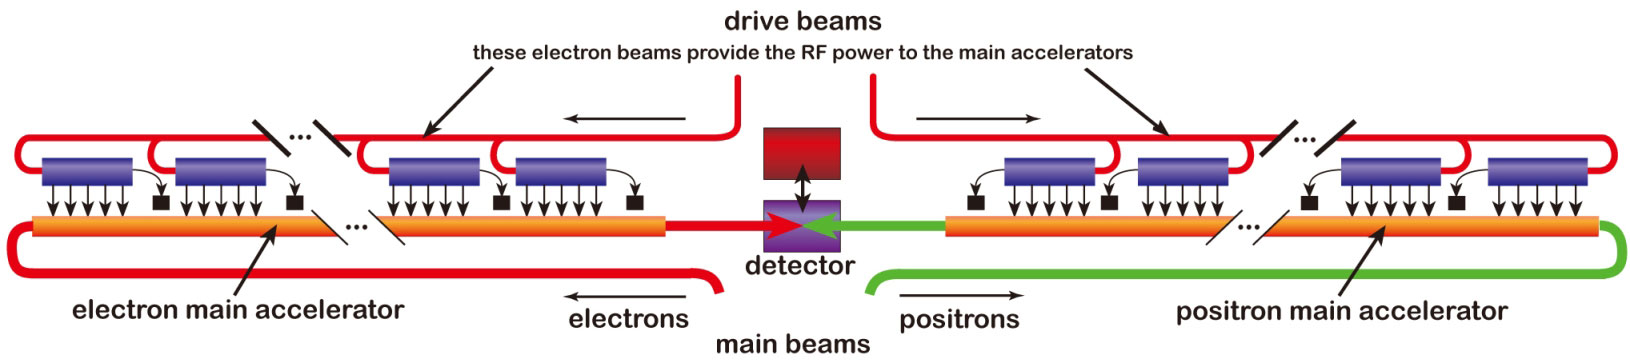
\includegraphics[width=\textwidth]{images/CLIC-layout.jpg}
\centering
\caption{Το σχεδιάγραμμα του \en{CLIC}}
\label{CLIClayout}
\end{figure}

Ο \en{CLIC} είναι μία από τις επιλογές για έναν μελλοντική επιταχυντή κατασκευασμένο στο \en{CERN}, το οποίο θα αποφασιστεί ανάλογα με τα μελλοντικά αποτελέσματα του \en{LHC}.

\section{\selectlanguage{greek}Το \en{Electron beam scanner}}



\chapter{Chapter Three Title}
\chapter{Σχετική βιβλιογραφία}

Στο κεφάλαιο αυτό παρουσιάζουμε σχετικές προσεγγίσεις και υλοποιήσεις στο πρόβλημα του αυτόματου προγραμματισμού και της παραγωγής κώδικα.
Επειδή είναι πρακτικά αναρίθμητες, θα επικεντρωθούμε σε αυτές που είναι σχετικές με τα αναδραστικά νευρωνικά δίκτυα και σε κάποιες που παρουσιάζουν ιδιαίτερο ενδιαφέρον.

\section{\en{Generating Sequence with Recurrent Neural Networks}}
Στην εργασία των \en{Graves et al.} παρουσιάζεται πως απλές δομές αναδραστικών νευρωνικών δικτύων με στοιχεία μνήμης \en{LSTM} μπορούν να χρησιμοποιηθούν για να παράξουν σύνθετες ακολουθίες, απλά προβλέποντας ένα στοιχείο της ακολουθίας τη φορά. 
Θεωρώντας τις προβλέψεις στοχαστικές, καινούριες ακολουθίες μπορούν να προκύψουν από ένα εκπαιδευμένο δίκτυο, δειγματοληπτώντας επαναληπτικά από την έξοδο του δικτύου και ύστερα ξανά-δίνοντας ως είσοδο στο δικτύου την δειγματοληπτημένη πρόβλεψη.
Με μία διαφορετική διατύπωση, αφήνουμε το δίκτυο να αντιμετωπίσει τις επινοήσεις του ως αληθινές, περίπου σαν έναν άνθρωπο ο οποίος ονειρεύεται. 
Αν και το σύστημα είναι ντετερμινιστικό, η στοχαστικότητα που εισάγεται δειγματοληπτώντας δημιουργεί μία κατανομή σε σχέση με τις ακολουθίες.
Αυτή η κατανομή είναι δεσμευμένη, αφού η εσωτερική αναπαράσταση του δικτύου, άρα και κατανομή προβλέψεων του, εξαρτάται από τις προηγούμενες εισόδους.

Η προσέγγιση αυτή επιδεικνύεται για κείμενο (όπου οι τιμές είναι διακριτές) και για <<\en{online}>>  χειρόγραφο κείμενο (όπου οι τιμές είναι πραγματικές).
Με τον όρο <<\en{online}>> εννοούμε ότι η γραφή αποτυπώνεται ως ακολουθία διανυσμάτων θέσης ενός μολυβιού -- σε αντίθεση με το <<\en{offline}>> στο οποίο έχουμε διαθέσιμη ολόκληρη την εικόνα του χειρόγραφου.
Το σύστημα που χρησιμοποιείται είναι μια συστάδα που αποτελείται από 7 επίπεδα αναδραστικών νευρωνικών δικτύων με 700 στοιχεία μνήμης \en{LSTM}.
Για την παραγωγή ακολουθιών κειμένου χρησιμοποιούνται τρία διαφορετικά σετ δεδομένων. Το Penn Treebank και το Wikipedia Hutter Prize για το γραπτό κείμενο και το <<\en{IAM online handwriting database}>>.
Το μοντέλο καταφέρνει να παράξει ακολουθίες τόσο ρεαλιστικές ώστε να είναι συχνά δύσκολο να τις ξεχωρίσει κανείς από πραγματικές, τουλάχιστον σε πρώτη όψη.
Στα αποτελέσματα είναι ορατή μια μεγάλης εμβέλειας δομή και συνοχή.

\begin{figure}[tph]
	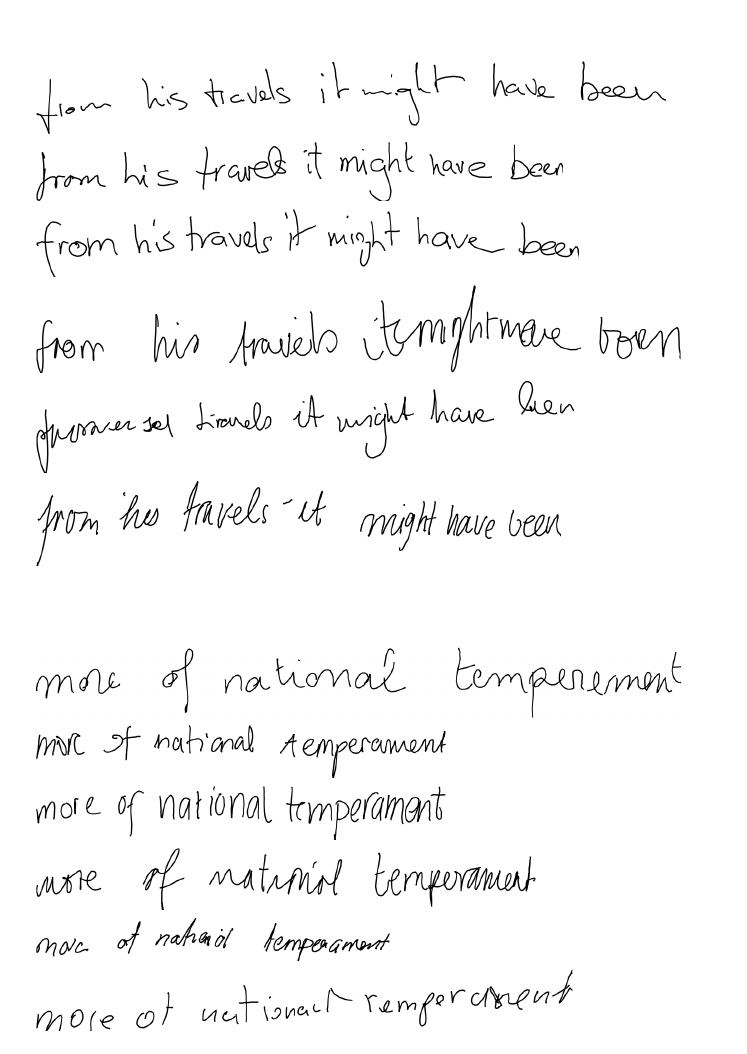
\includegraphics[width=\textwidth, keepaspectratio]{images/handwriting.png}
	\centering 
	\caption{Ένα τυπικό δομικό διάγραμμα επιτηρούμενης εκμάθησης.}
	\label{fig:training}
\end{figure}

Επιπρόσθετα, βασισμένοι στην προηγούμενη δομή, οι \en{Graves et al.} σχεδιάζουν ένα σύστημα παραγωγής χειρόγραφου κειμένου το οποίο μπορεί να γράψει αυτό που του ζητάμε.
Αυτό γίνεται με την προσθήκη ενός διανύσματος της πρότασης που θέλουμε να γράψουμε, το οποίο δίνεται στο σύστημα πρόβλεψης την ώρα της παραγωγής, αφού προφανώς εκπαιδευτεί σε σχετικά προβλήματα.
Η απόφαση για το πότε και πως θα γραφεί κάθε χαρακτήρας αφήνεται στο νευρωνικό δίκτυο και τα αποτελέσματα είναι αρκετά ικανοποιητικά ώστε να είναι και πάλι δύσκολο να διακριθεί αν τα <<χειρόγραφα>> ανήκουν σε κάποιον άνθρωπο ή στο σύστημα.

\section{\en{Inferring Algorithmic Patterns with Stack-Augmented Recurrent Nets}}

Οι \en{Joulin et al.} στην έρευνα τους εξετάζουν τα όρια των \en{"state of the art" Deep Learning} προσεγγίσεων.
Πιο συγκεκριμένα, εξετάζονται τα απλούστερα προβλήματα πρόβλεψης ακολουθιών που είναι πέρα από τις δυνατότητες εκμάθησης των τυπικών αναδραστικών δικτύων: αλγοριθμικά παραγμένες ακολουθίες που μπορούν να μαθευτούν μόνο από συστήματα με δυνατότητα μνήμης και απαρίθμησης.
Για παράδειγμα η σχέση $a^nb^n, n > 0$ μπορεί να παράξει την ακολουθία \en{aab\textbf{ba}aab\textbf{bba}b\textbf{a}aaaab\textbf{bbbb}}, όπου με έντονη γραμματοσειρά σημειώνονται τα στοιχεία της ακολουθίας που μπορούν να προβλεφθούν ντετερμινιστικά.

Εξετάζονται 4 διαφορετικά μοντέλα: ένα απλό αναδραστικό νευρωνικό δίκτυο, ένα \en{RNN} με στοιχεία μνήμης \en{LSTM} και 2 \en{RNN} με εξωτερική μνήμη.
Η εξωτερική μνήμη είναι για το ένα μοντέλο μια διπλά συνδεδεμένη λίστα και για το άλλο μοντέλο μια στοίβα. Όλα τα μοντέλα εκπαιδεύονται με τον αλγόριθμο \en{SGD}.
Τα μοντέλα με την εξωτερική μνήμη μαθαίνουν να χρησιμοποιούν τις θεωρητικά απείρου μήκους εξωτερικές μνήμες τους, με στοιχειώδεις εντολές (\en{push, pop, insert, no-op}). 

Τελικώς δείχνουν πως μερικοί βασικοί αλγόριθμοι μπορούν να μαθευτούν από ακολουθιακά δεδομένα χρησιμοποιώντας \en{RNNs} με μνήμη. Τα μοντέλα με εξωτερική μνήμη ξεπερνούν σε επιδόσεις τα υπόλοιπα μοντέλα. Οι συγγραφείς υποσημειώνουν πως είναι σημαντικό να μεγαλώσουμε την πολυπλοκότητα του μοντέλου με δομημένο τρόπο και πως η δομή των νευρωνικών δικτύων θα πρέπει να μαθαίνεται από τα δεδομένα και να μην προαποφασίζεται.

\section{\en{A Synthetic Neural Model for General Purpose Code Generation}}

Στην έρευνα τους, οι \en{Yin et al.} ασχολούνται με την αυτόματη μετατροπή εντολών φυσικής γλώσσας σε πηγαίο κώδικα γλωσσών γενικής χρήσης.
Σε αντίθεση με την πλειοψηφία των μεθόδων που απαντώνται στην βιβλιογραφία, που αντιμετωπίζουν το πρόβλημα χωρίς να λαμβάνουν υπ' όψιν την γραμματική της τελικής γλώσσας, οι ερευνητές προτείνουν ένα μοντέλο στο οποίο η γραμματική είναι γνωστή \en{a priori}.

Το συντακτικά-οδηγούμενο νευρωνικό μοντέλο παραγωγής κώδικα που προτείνεται βασίζεται σε ένα γραμματικό μοντέλο που ορίζει την παραγωγή ενός \en{Abstract Syntax Tree} σε ακολουθίες στοιχειωδών δράσεων.
Οι δράσεις αυτές χωρίζονται κανόνες παραγωγής κώδικα και σε εντολές.
Με αυτό τον τρόπο το μοντέλο δε χρειάζεται να μάθει την γραμματική από τα περιορισμένα σε ποσότητα δεδομένα εκμάθησης.
Το αναδραστικό νευρωνικό δίκτυο που χρησιμοποιείται βασίζεται σε στοιχεία \en{LSTM} με τροποποίηση, ώστε να λαμβάνεται υπ' όψιν η αναδρομική φύση των γλωσσών προγραμματισμού.
Η δομή του συστήματος γίνεται σύμφωνα με αρχιτεκτονική \en{encoder-decoder RNN with attention} \cite{Bahdanau2014}, τεχνική η οποία γνωρίζει μεγάλη χρήση και επιτυχία τα λίγα χρόνια ύπαρξης της.
Για την εκπαίδευση <<δείχνουμε>> στο νευρωνικό κομμάτια κώδικα, μετατρέπονται σε \en{ASTs}και από εκεί σε κώδικα σύμφωνα την γραμματική που υποδεικνύεται.

Το μοντέλο ξεπερα τις \en{state of the art} προσεγγίσεις νευρωνικών δικτύων των Ling και των Dong\cite{} and Lapata\cite{} στο \en{Hearthstone dataset} με παραγόμενη γλώσσα την \en{Python}.
Συμπεραίνεται έτσι, η σημαντικότητα της γραμματικής της γλώσσας σε σχέση με τις επιδόσεις. 

\section{\en{End-to-End Memory Networks}}

Οι Sukhbaatar et al., παρουσιάζουν ένα ευέλικτο νευρωνικό μοντέλο με μεγάλη εξωτερική μνήμη. 
Το μοντέλο σε αντίθεση με αντίστοιχες εργασίες δικτύων με μνήμη εκπαιδεύεται <<\en{end-to-end}>>, που, στα πλαίσια της εκπαίδευσης μοντέλων νευρωνικών δικτύων, σημαίνει πως το μοντέλο εκπαιδεύεται σε μια ενιαία διαδικασία και απλά του δίνονται οι είσοδοι και οι σωστές έξοδοι, χωρίς επιπρόσθετη εργασία για δημιουργία και ρύθμιση χαρακτηριστικών. Οι επιδόσεις του συστήματος εξετάζονται σε προβλήματα συνθετικών ερωταπαντήσεων και σε προβλήματα μοντελοποίησης φυσικής γλώσσας.

Το σύστημα δέχεται ένα σετ εισόδων, μια ερώτηση και εξάγει μία απάντηση. 
Το σετ εισόδων αποθηκεύεται στη μνήμη σε μορφή εσωτερικών αναπαραστάσεων. Για κάθε ερώτηση υπολογίζεται ένας δείκτης που εκφράζει κατά πόσο αντιστοιχεί η ερώτηση με τα στοιχεία της μνήμης.
Από τις εισόδους, επιπρόσθετα, υπολογίζεται και μία αναπαράσταση της αναμενόμενης εξόδου.
Η τελευταία σε συνδυασμό με τον δείκτη συσχέτισης ερώτησης-μνήμης χρησιμοποιείται για την εξαγωγή της τελικής απάντησης. Ολόκληρο το σύστημα είναι παραγωγίσιμο, οπότε μπορούμε να χρησιμοποιήσουμε τις τυπικές μεθόδους για την εκμάθηση του.

Για να εξετάσουμε τις επιδόσεις στην μοντελοποίηση φυσικής γλώσσας (με την οποία ασχολούμαστε επειδή βρίσκεται πιο κοντά στο πρόβλημα του αυτόματου προγραμματισμού) χρησιμοποιούμε τα \en{Penn Treebank Dataset} και \en{Text8 dataset}. Το δίκτυο μνήμης το οποίο εξετάσαμε ξεπερνά σε επιδόσεις διατάξεις \en{RNN} και \en{LSTM}. Αξιοσημείωτο είναι πως το νευρωνικό μοντέλο μνήμης έχει σημαντικά λιγότερες παραμέτρους από το αντίστοιχο \en{LSTM}. Σε ακόμα ένα πείραμα, έτσι, υποδεικνύεται η σημαντικότητα ύπαρξης εξωτερικής μνήμης στις διατάξεις εκμάθησης.

\section{\en{Neuro Symbolic Program Synthesis}}

Στην έρευνα τους οι \en{Parisotto et al.} ασχολούνται με ένα νευρωνικό μοντέλο σύνθεσης προγραμμάτων με σκοπό την επεκτασιμότητα και την εύκολη εξέταση της ορθότητας του παραγώμενου μοντέλου.
Σε αντίθεση με την πλειοψηφία των προσεγγίσεων στη σύγχρονη βιβλιογραφία, όπου ο χώρος αναζήτησης είναι σύμβολα της γλώσσας την οποία παράγουμε, εδώ, ο χώρος αναζήτησης είναι υποπρογράμματα που μαθαίνει το σύστημα κατά τη διάρκεια της μάθησης. Το όνομα που δίνεται στο υποσύστημα παραγωγής είναι \en{Recursive-Reverse-Recursive Neural Network (R3NN)}.


Το υποσύστημα παραγωγής εξάγει αναπαραστάσεις υποπρογραμμάτων σε μορφές δέντρων, στις οποίες κάθε στοιχείο είναι είτε κανόνας παραγωγής είτε σύμβολο, διαδικασία η οποία χωρίζεται σε 3 μέρη.
Αρχικά δεδομένου ενός τέτοιου δέντρου, δίνεται ένα διάνυσμα αναπαράστασης σε κάθε φύλλο του.
Ύστερα, το δέντρο διαβάζεται προς τα πάνω, ώστε να δοθεί μία αναπαράσταση ολόκληρου του δέντρου στη ρίζα του.
Τέλος επαναλαμβάνεται το προς τα κάτω πέρασμα ώστε να δοθεί σε κάθε φύλλο μια αναπαράσταση ολόκληρου του δέντρου.
Με αυτό τον τρόπο κάθε φύλλο έχει πληροφορία για τα υπόλοιπα φύλλα και για την συνολική λειτουργικότητα του δέντρου. Τα προγράμματα στο σετ δεδομένων χωρίζονται σε στοιχειώδη βήματα για να επεξεργαστούν με τον τρόπο που περιγράψαμε παραπάνω. Τα δεδομένα εκπαίδευσης σε αυτή την περίπτωση αποτελούνται από αναπαραστάσεις εισόδων και εξόδων που δίνονται στο σύστημα παραγωγής με σε κάθε φύλλο του δέντρου.

Το σύστημα εξετάζεται στη δημιουργία προγραμμάτων διαχείρισης αλφαριθμητικών ακολουθιών. Καταφέρνει σε ένα βαθμό και να επεκτείνει προγράμματα που ήδη έχει <<δει>> ώστε να συμπεριλαμβάνουν καινούρια ζευγάρια εισόδου εξόδου αλλά και να δημιουργήσει καινούρια προγράμματα για καινούριου είδους ζευγάρια εισόδου εξόδου. Η επεκτασιμότητα που παρουσιάζει το σύστημα αυτό, με την έννοια ότι μπορεί να ξεκινήσει από κάποια προγράμματα και ύστερα να τα εμπλουτίσει είναι ένα σημαντικό και αισιόδοξο στοιχείο στην κατεύθυνση του αυτόματου προγραμματισμού. 


\chapter{Chapter Four Title}
\chapter{\selectlanguage{greek}Μεθοδολογία}
Στο κεφάλαιο αυτό περιγράφεται η προσέγγιση μας στην παραγωγή κώδικα χρησιμοποιώντας αναδραστικά νευρωνικά δίκτυα.
Εμπνεόμαστε από το \en{blog post} του \en{Andrej Karpathy}\footnote{\en{\url{http://karpathy.github.io/2015/05/21/rnn-effectiveness/}}}, στο οποίο χρησιμοποιείται μια σχετικά απλή δομή \en{RNN} με \en{LSTM} στοιχεία η οποία εκπαιδεύεται στα έργα του \en{Shakespeare}, κατά χαρακτήρα, και παράγει παρόμοιο κείμενο.
Χρησιμοποιούμε το ίδιο μοντέλο, εκπαιδευμένο σε κώδικα \en{JavaScript}.
Προτείνουμε μία επέκταση του προηγούμενου μοντέλου που χρησιμοποιεί \en{a priori} γνώση για τον κώδικα, με σκοπό να βελτιώσουμε τις επιδόσεις πρόβλεψης του μοντέλου και να εξετάσουμε τη διαίσθηση πως με περισσότερη χρήσιμη πληροφορία ο παραγώμενος κώδικας θα είναι ποιοτικότερος.
Εξετάζουμε τα μοντέλα σε 2 διαφορετικά σετ δεδομένων.
Παρακάτω ακολουθεί αναλυτική παρουσίαση της μεθόδου, την οποία χωρίζουμε σε 3 στάδια: 1) προ-επεξεργασία, 2) εκπαίδευση και 3) παραγωγή \en{(generation)}.

\section{Τα μοντέλα}

\subsection{Τα Αναδραστικά Νευρωνικά Δίκτυα ως Μοντέλα Παραγωγής}
Ο στόχος της μοντελοποίησης γλώσσας κατά χαρακτήρα (χωρίς να αναφερόμαστε απαραίτητα στην προγραμματιστική γλώσσα) είναι να προβλέψει τον επόμενο χαρακτήρα σε μία ακολουθία.
Δεδομένης μιας εκπαιδευτικής ακολουθίας $(x_1, x_2, ..., x_T)$, τα αναδραστικά νευρωνικά δίκτυα χρησιμοποιούν τις εξόδους τους $(ο_1, ο_2, ..., ο_T)$ για να πάρουν κατανομές προβλέψεων της μορφής $P(x_{t+1}|x_{\leq{t}}) = P(softmax(o_t))$, όπου η κατανομή <<\en{softmax}>> ορίζεται: $P(softmax(o_t) = j) = exp(o_t^{(j)}/\sum_k exp(o_t^{(k)})$.
Ο στόχος που χρησιμοποιείται για την μοντελοποίηση της γλώσσας είναι η μεγιστοποίηση της λογαριθμικής πιθανότητας της εκπαιδευτικής ακολουθίας $\sum_{t=0}^{T-1}logP(x_{t+1}|x_{\leq{t}})$.
Όπως και στην εργασία των \en{Graves et al.} \cite{Graves2013}, εισάγουμε στοχαστικότητα δειγματοληπτώντας από την έξοδο του νευρωνικού δικτύου και δίνοντας την τυχαία επιλογή μας ως είσοδο, την επόμενη χρονική στιγμή.

\subsection{Μοντέλο \en{char-rnn}}

Το πρώτο μοντέλο είναι ένα αναδραστικό νευρωνικό δίκτυο με 3 κρυμμένα επίπεδα στοιχείων \en{LSTM}.
Κάθε στιγμή το σύστημα δέχεται χαρακτήρες κώδικα σε μορφή διανυσμάτων  \en{\textit{one-hot}} (διανύσματα με όλα τα στοιχεία 0 εκτός από το στοιχείο εκείνο που αντιστοιχεί στον χαρακτήρα και παίρνει την τιμή 1).
Ενημερώνει την εσωτερική του κατάσταση και εξάγει μια πρόβλεψη για τον επόμενο χαρακτήρα.
Οι προβλέψεις του \en{char-rnn} είναι κατανομές του λεξιλογίου, που στην περίπτωση μας αποτελείται από χαρακτήρες.
Έστω ότι έχουμε το λεξιλόγιο \en{A, B, C, T}.
Αν θέλουμε να εκπαιδεύσουμε το σύστημα στην ακολουθία <<\en{BCAT}>>, δίνουμε ένα χαρακτήρα τη φορά και θέλουμε να μεγιστοποιηθούν οι υπογραμμισμένες πιθανότητες (Σχήμα \ref{fig:char-rnn}). Στη διαδικασία της παραγωγής (διακεκομμένες γραμμές) δειγματοληπτούμε από τις κατανομές εξόδου για να αποφασίσουμε τον επόμενο χαρακτήρα που δίνεται στο σύστημα. 


\begin{figure}[h]
	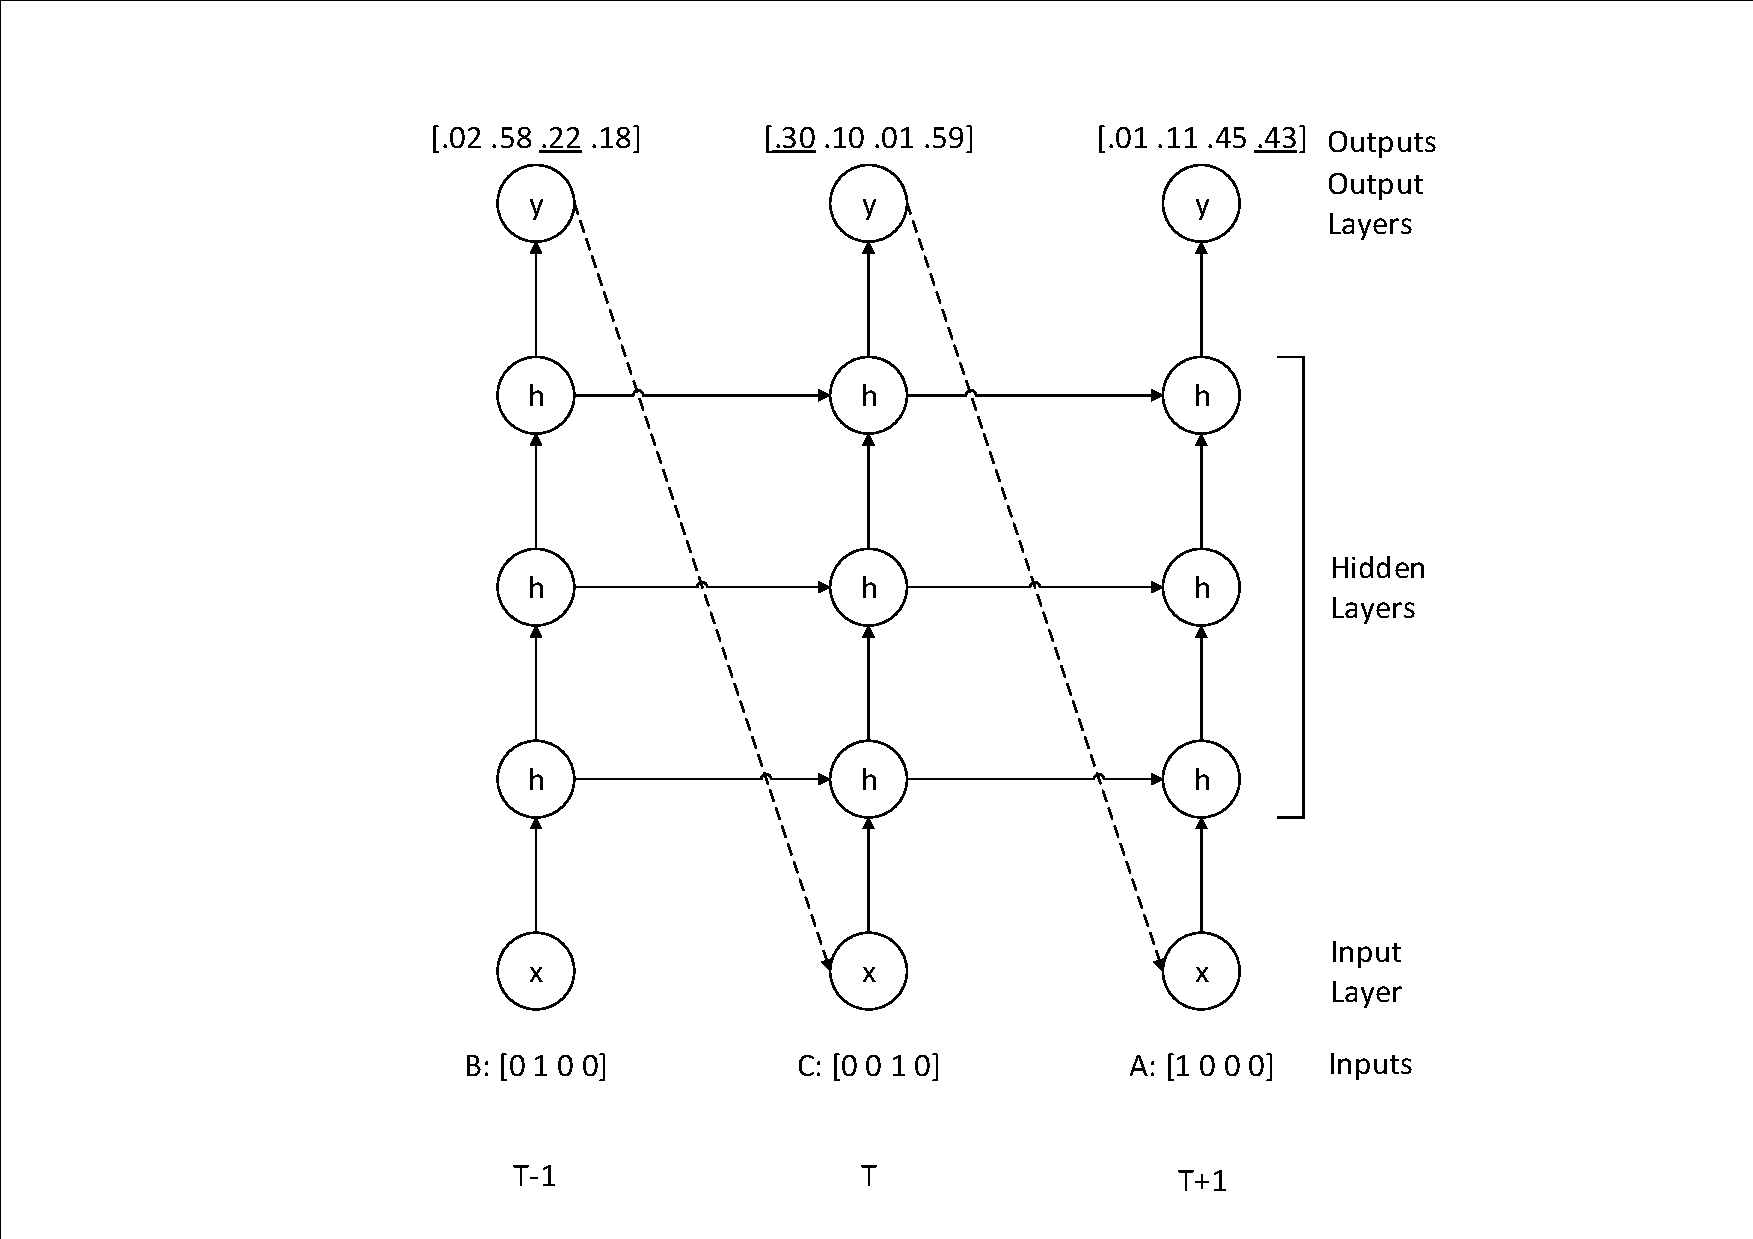
\includegraphics[width=\textwidth, trim = 4 4 4 4, clip, keepaspectratio]{images/char-rnn.pdf}
	\centering 
	\caption{Το μοντέλο \en{char-rnn} ανεπτυγμένο στο χρόνο.}
	\label{fig:char-rnn}
\end{figure}

\subsection{Μοντέλο \en{labeled-char-rnn}}

Το δεύτερο μοντέλο είναι επίσης ένα αναδραστικό νευρωνικό δίκτυο με 3 κρυμμένα επίπεδα στοιχείων \en{LSTM}. 
Εκτός από ακολουθίες χαρακτήρων, το μοντέλο αυτό δέχεται και πληροφορία για το είδος του χαρακτήρα. 
Αντίστοιχα οι έξοδοι του, εκτός από προβλέψεις για τον χαρακτήρα, περιέχουν και προβλέψεις για το είδος του χαρακτήρα. Με τον τρόπο αυτό θα εξετάσουμε κατά πόσο τα \en{RNNs} μπορούν να εκμεταλλευτούν \en{a priori} γνώσεις για τον κώδικα. Σημειώνεται πως η συνάρτηση επιδόσεων αυτού του μοντέλου είναι γραμμικός συνδυασμός των επιμέρους επιδόσεων πρόβλεψης χαρακτήρα και είδους χαρακτήρα.

Έστω το λεξιλόγιο \en{A, B, C, T}.
Έστω επίσης πως δίνουμε το είδος των χαρακτήρων αυτών στο σύστημα με βάση το αν είναι φωνήεντα ή σύμφωνα.
Για την εκπαιδευτική ακολουθία  <<\en{BCAT}>> δίνουμε την κατάλληλη είσοδο όπως στο σχήμα \ref{fig:l-char-rnn}.
Θέλουμε να μεγιστοποιηθούν και πάλι οι υπογραμμισμένες πιθανότητες. Για την παραγωγή του επόμενου χαρακτήρα και του είδους του, δειγματοληπτούμε από κάθε κατανομή εξόδου ξεχωριστά.

\begin{figure}[h]
	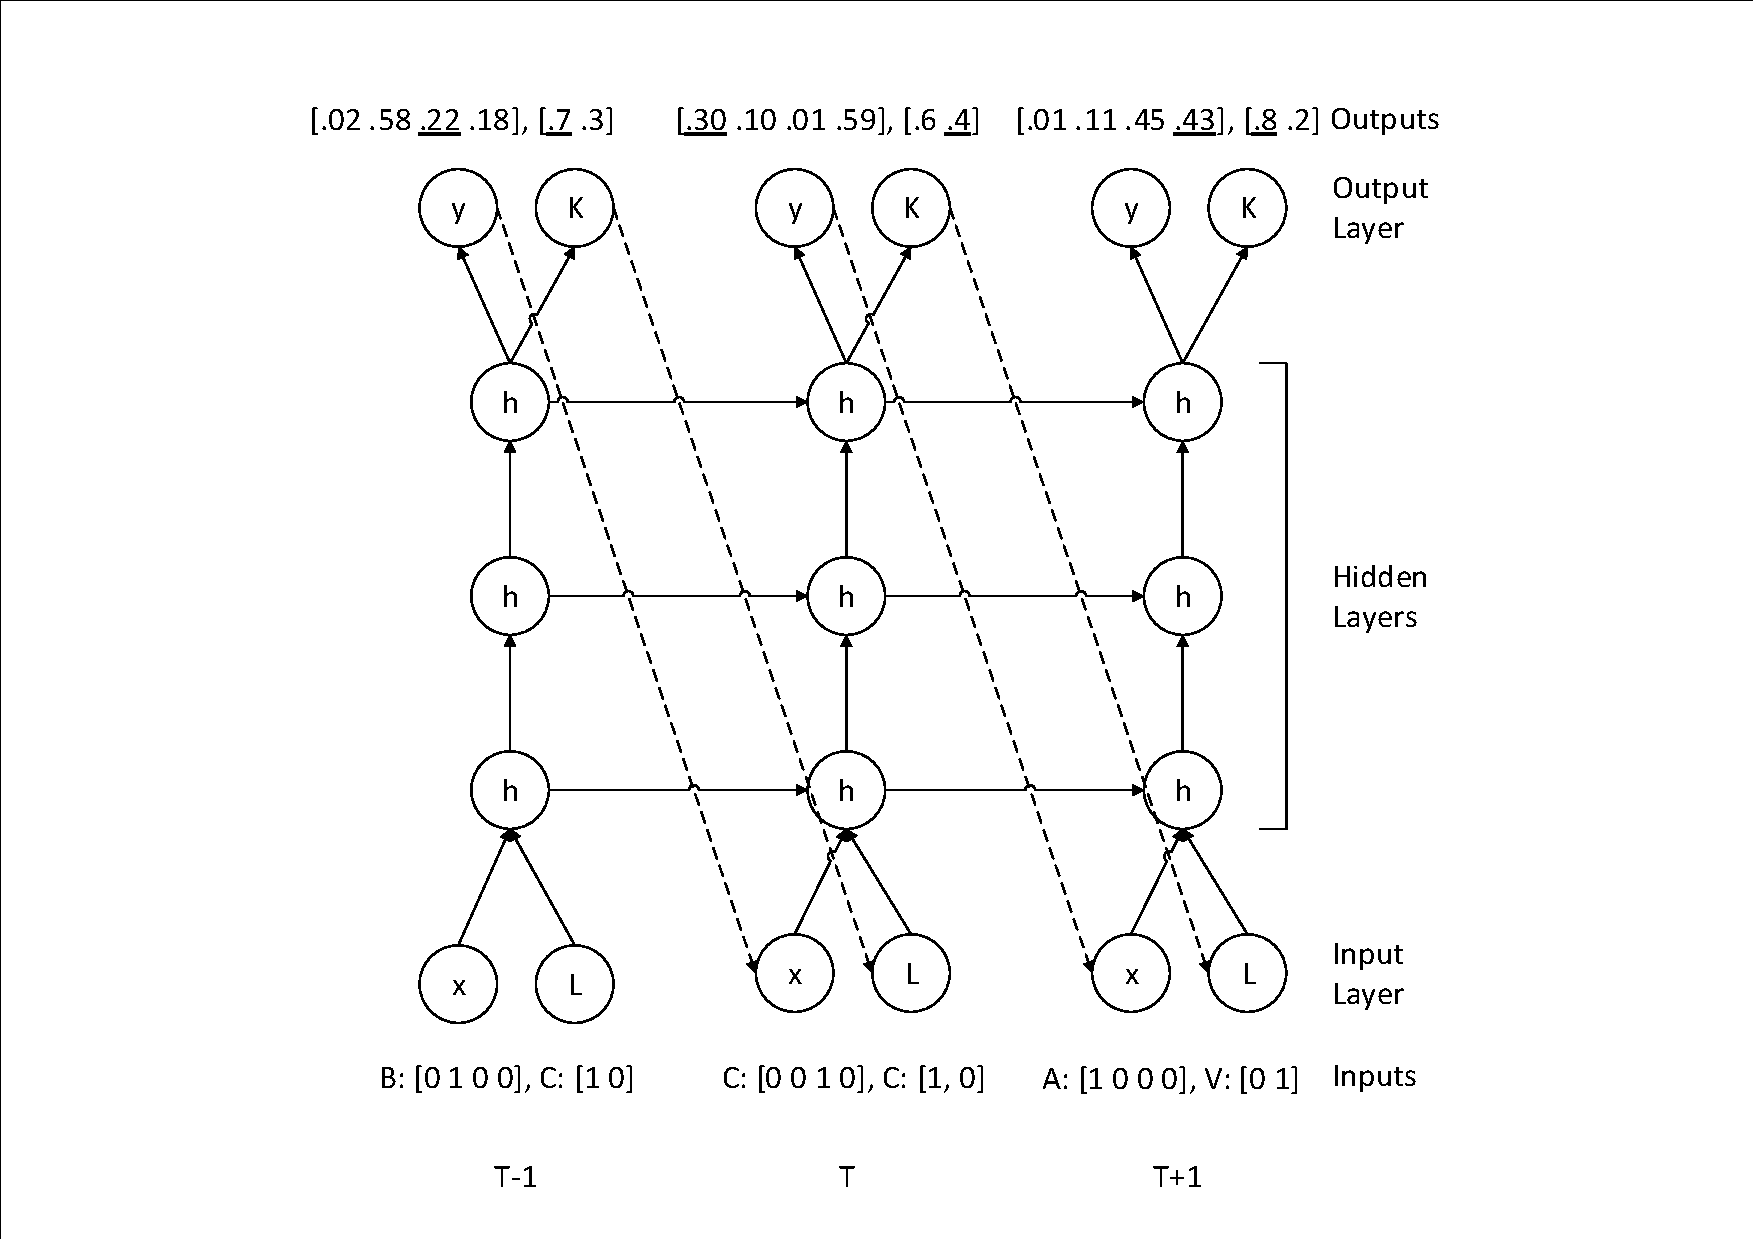
\includegraphics[width=\textwidth, trim = 4 4 4 4, clip, keepaspectratio]{images/l-char-rnn.pdf}
	\centering 
	\caption{Το μοντέλο \en{labeled-char-rnn} ανεπτυγμένο στο χρόνο.}
	\label{fig:l-char-rnn}
\end{figure}

\section{Προ-επεξεργασία}

Ο κορμός της διαδικασίας της προ-επεξεργασίας είναι ίδιος και για τα δύο σετ δεδομένων. 
Αρχικά αναζητούμε τα αρχεία με κατάληξη <<\en{.js}>> διασχίζοντας σειριακά όλους τους φακέλους των \en{projects}, εκτός από αυτούς που αφορούν \en{testing} και \en{localization}.
Ο έλεγχος για το τελευταίο γίνεται απλοϊκά, ελέγχουμε δηλαδή αν οι φάκελοι φέρουν τα συνήθη ονόματα που χρησιμοποιούνται για τέτοιου είδους φακέλους.
Ο μη ενδελεχής έλεγχος καταφέρνει να αφαιρέσει την πλειοψηφία των επαναλαμβανόμενων αρχείων αφήνοντας ένα μικρό ποσοστό να περάσει.
Αυτό έχει ως αποτέλεσμα να εμπλουτιστεί η εκπαίδευση του νευρωνικού, χωρίς όμως να μονοπωλείται το ενδιαφέρον από αρχεία που περιέχουν τετριμμένο κώδικα.
Στη συνέχεια, με τη βοήθεια ενός εργαλείου ανάλυσης της σύνταξης και γραμματικής προγραμματιστικών γλωσσών (ονόματι \en{\textit{linguist}}\footnote{\en{\url{https://github.com/github/linguist/}}}) προχωράμε στο περαιτέρω φιλτράρισμα αρχείων.
Συγκεκριμένα, εξαιρούμε αρχεία που έχουν την κατάληξη <<\en{.js}>> αλλά δεν είναι αρχεία κειμένου και αρχεία που είναι αυτόματα παραγώμενα και αποτελούν παραπροϊόν της διαδικασίας ανάπτυξης λογισμικού σε \en{JavaScript}.

\selectlanguage{english}
\lstinputlisting[language=JavaScript, caption={\tg{Αρχείο κώδικα πριν το }\en{minification}}]{code/beforemin.js}
\selectlanguage{greek}

\selectlanguage{english}
\lstinputlisting[language=JavaScript, caption={\tg{Αρχείο κώδικα μετά το }\en{minification}}]{code/aftermin.js}
\selectlanguage{greek}

Αφού επιλέξουμε τα αρχεία τα οποία θα αποτελούν το σετ δεδομένων μας προχωράμε στη διαδικασία της ελαχιστοποίησης του κώδικα (\en{minification, minimisation}).
Η ελαχιστοποίηση κώδικα, είναι η διαδικασία αφαίρεσης περιττών χαρακτήρων από των πηγαίο κώδικα, χωρίς να αλλάζει η λειτουργικότητά του. Τέτοιοι χαρακτήρες είναι τα κενά, τα σύμβολα αλλαγής παραγράφου, τα σχόλια και άλλα. Εδώ χρησιμοποιήθηκε το εργαλείο \en{\textit{jsmin}}\footnote{\en{\url{http://www.crockford.com/javascript/jsmin.html}}}. Οι κώδικες 4.1, 4.2 δείχνουν ένα αρχείο κώδικα πριν και μετά το \en{minification}.

Με την επιλογή αυτή προσπαθούμε να αφαιρέσουμε την περιττή πληροφορία απο τα δεδομένα μας, ώστε να είναι πιο εύκολο για το μοντέλο να αποτυπώσει τις σημαντικές σχέσεις ανάμεσα στους διάφορους χαρακτήρες.
Μετά το \en{minification} προσθέτουμε 2 ειδικούς χαρακτήρες για την αρχή και το τέλος κάθε αρχείου. Σημειώνεται πως θεωρούμε πως τα αρχεία ειναι \en{extended ASCII} κωδικοποιημένα και στην ουσία διαβάζουμε \en{bytes}.

Για την εκπαίδευση του μοντέλου \en{labeled-char-rnn} χρειάζεται να προετοιμάσουμε με ανάλογο τρόπο την πληροφορία για το είδος των χαρακτήρων. Για το σκοπό αυτό, χρησιμοποιούμε ένα άλλο εργαλείο ανάλυσης σύνταξης και γραμματικής προγραμματιστικών γλωσσών που φέρει το όνομα \en{\textit{pygments}}\footnote{\en{\url{http://pygments.org}}}.
Η επιλογή για τον διαχωρισμό των ειδών βασίζεται στα αυθαίρετα συντακτικά δέντρα (\en{abstract syntax trees}) της \en{JavaScript}, είναι όμως απλουστευμένη και δε χρησιμοποιεί δομές δέντρων, αλλά απλών διανυσμάτων.
Ο διαχωρισμός των χαρακτήρων γίνεται ανάμεσα στις ακόλουθες κλάσεις: \en{(\textbf{K}eyword, \textbf{N}umber, \textbf{R}egex, \textbf{S}tring, \textbf{O}perator, \textbf{P}unctuator, \textbf{I}dentifier).}

Οι χαρακτήρες και τα είδη τους αποθηκεύονται ως λίστες από αλφαριθμητικά στοιχεία ώστε να είναι διαθέσιμα ανά πάσα στιγμή στην εκπαιδευτική διαδικασία.
Προφανώς υπάρχει χρονική αντιστοιχία μεταξύ των αρχείων που περιέχουν της ακολουθίες χαρακτήρων με τα αρχεία που περιέχουν το είδος κάθε χαρακτήρα, όπως στα παραδείγματα του πίνακα \ref{label-example}.
Συνηθίζεται σε τέτοιου είδους προβλήματα να <<\tg{ανακατεύονται}>> οι ακολουθίες αλφαριθμητικών χαρακτήρων με σκοπό την .
Στα προβλήματα μάθησης έχουμε τη δυνατότητα να <<\tg{ανακατεύουμε}>> το σετ δεδομένων με σκοπό την γρηγορότερη/καλύτερη εκπαίδευση των μοντέλων.
Επειδή το ζητούμενο μας στη διπλωματική αυτή είναι η παραγωγή κώδικα, και η σειρά των ακολουθιών είναι άρρηκτα συνδεδεμένη με τη λειτουργικότητα και την ουσία των προγραμμάτων, δεν προχωράμε σε αυτή την επιλογή.  

\begin{table}[]
\centering
\caption{Παράδειγμα αντιστοιχίας χαρακτήρων με το είδος τους σε μια ακολουθία}
\label{label-example}
\begin{tabularx}{\textwidth}{|l|XXXXXXXXXXXXXXXXXXXXX|}
\hline
\en{String 1} & \en{v} & \en{a} & \en{r} &   & \en{a} & = & 1 & \en{;} & \en{f} & \en{u} & \en{n} & \en{c} & \en{t} & \en{i} & \en{o} & \en{n} &   & \en{f} & \en{(} & \en{A} & \en{)} \\ \hline
\en{Label 1}  & \en{K} & \en{K} & \en{K} & \en{P} & \en{I} & \en{O} & \en{N} & \en{P} & \en{K} & \en{K} & \en{K} & \en{K} & \en{K} & \en{K} & \en{K} & \en{K} & \en{P} & \en{I} & \en{P} & \en{I} & \en{P} \\ \hline
\hline
\en{String 2} & \{ & \en{r} & \en{e} & \en{t}  & \en{u} & \en{r} & \en{n} &  & < & \en{o} & \en{k} &  > & \en{;} & \} & \en{c} & = & \en{f} & \en{(} & \en{1} &\en{0} & \en{)} \\ \hline
\en{Label 2}  & \en{P} & \en{K} & \en{K} & \en{K} & \en{K} & \en{K} & \en{K} & \en{P} & \en{S} & \en{S} & \en{S} & \en{S} & \en{P} & \en{P} & \en{I} & \en{O} & \en{I} & \en{P} & \en{N} & \en{N} & \en{P} \\ \hline
\end{tabularx}
\end{table}

\section{Εκπαίδευση}


Η εκπαίδευση γίνεται στο \en{training set} του καθενός από τα δύο σετ δεδομένων. 
Οι χαρακτήρες δίνονται ως \en{\textit{one-hot}} διανύσματα, με μήκος όσο και οι διαφορετικοί χαρακτήρες του σετ δεδομένων.
Χρησιμοποιείται η τεχνική του \en{dropout}, ενώ ο αλγόριθμος που χρησιμοποιείται για την ελαχιστοποίηση του λάθους είναι ο \en{TBPTT}.
Η συνάρτηση λάθους είναι η \en{cross-entropy loss function}: $\sum_x p(x) \log{q(x)}$, όπου $p(x)$ είναι η πραγματική κατανομή των χαρακτήρων και $q(x)$ η προβλεπόμενη κατανομή χαρακτήρων του μοντέλου.
Η συνάρτηση αυτή χρησιμοποιείται στην πλειοψηφία της σύγχρονης βιβλιογραφίας και εμπειρικά έχει καλά αποτελέσματα στην εκπαίδευση των αναδραστικών νευρωνικών δικτύων.
Εξίσου ευρεία χρήση συναντά και η συνάρτηση \en{\textit{rmsprop}} που χρησιμοποιούμε για τη βελτιστοποίηση του \en{gradient descent}.

Η εκπαίδευση του αναδραστικού νευρωνικού δικτύου γίνεται, πιο περιγραφικά ως εξής: δείχνουμε στο νευρωνικό δίκτυο ακολουθίες σταθερού μήκους, το οποίο προαποφασίζεται της εκπαίδευσης.
Ως αληθείς απαντήσεις δίνουμε ένα διάνυσμα ίσου μήκους με το προηγούμενο που περιέχει τους χαρακτήρες της επόμενης χρονικής στιγμής (κύλιση του διανύσματος κατά μία θέση).
Στην περίπτωση του μοντέλου  \en{labeled-char-rnn} με όμοιο τρόπο δίνονται και οι πληροφορίες σχετικά με το είδος των χαρακτήρων, μαζί με τους αντίστοιχους χαρακτήρες.
Με σκοπό την παραλληλοποίηση του προγράμματος, δίνουμε πολλά τέτοια παραδείγματα ταυτόχρονα.

Συνολικά εκπαιδεύουμε 4 διαφορετικά μοντέλα. Για κάθε \en{dataset} το αντίστοιχο \en{char-rnn} και \en{labeled-char-rnn} μοντέλο.
Για την εκπαίδευση των μοντέλων, πρέπει να αποφασιστεί ένα σύνολο παραμέτρων, που φέρουν σημαντική αξία για τις τελικές επιδόσεις του μοντέλου και την διάρκεια της εκπαίδευσης. Αυτές είναι:

\begin{itemize} 
\item Μήκος ακολουθίας \en{(Sequence length)}: Ο αριθμός χαρακτήρων που περιέχει μία ακολουθία.
\item Μέγεθος παρτίδας \en{(Batch size)}: Ο αριθμός των εκπαιδευτικών ακολουθιών που δίνονται παράλληλα στο μοντέλο.
\item Μέγεθους κρυμμένων επιπέδων \en{(Hidden state size)}: Ο αριθμός των στοιχείων \en{LSTM} που απαρτίζουν κάθε κρυφό επίπεδο.
\item Πιθανότητα \en{dropout}: Η πιθανότητα να κρατηθεί ένα στοιχείο στη διάρκεια τη εκπαίδευσης.
\item Αριθμός εποχών \en{(Epoch number)}: Ο αριθμός <<περασμάτων>> του τεστ δεδομένων.
\item Ρυθμός εκμάθησης \en{(Learning rate)}: Πόσο γρήγορα μαθαίνει το σύστημα από τα λάθη του.

\end{itemize}

Για την στρατηγική επιλογής και την ακριβή τιμή των υπερ-παραμέτρων θα μιλήσουμε στο Κεφάλαιο 5.

\section{Παραγωγή}

Το μοντέλο που επιλέγουμε για καθένα από τα πειράματα αποφασίζεται σύμφωνα με τις επιδόσεις του στην μετρική λάθους της εκπαίδευσης.
Για να είναι ευκολότερα ερμηνεύσιμα τα αποτελέσματα της εκπαίδευσης, θα χρησιμοποιούμε και την μετρική της <<\tg{ευστοχίας}>>.
Η ευστοχία είναι το ποσοστό επιτυχημένων προβλέψεων επόμενου χαρακτήρα σε μία παρτίδα.

Η διαδικασία παραγωγής κώδικα που περιγράψαμε γενικεύεται και για τα μοντέλα που περιέχουν πληροφορία για το είδος των χαρακτήρων.
Μπορούμε δηλαδή να δειγματοληπτούμε από την προβλεπόμενη κατανομή για τα είδη των χαρακτήρων και να χρησιμοποιούμε το αποτέλεσμα ως επόμενη είσοδο.
Μπορούμε επίσης να οδηγήσουμε έμμεσα το σύστημα, αρχικοποιώντας το με κώδικα της επιλογής μας. Αυτό αλλάζει την εσωτερική κατάσταση του μοντέλου και το <<προϊδεάζει>> για το τι κώδικας μπορεί να ακολουθεί. 
Επιπρόσθετα, κατά τη διάρκεια της δειγματοληψίας έχουμε τη δυνατότητα να επηρεάσουμε την κατανομή που προτείνει το μοντέλο.
Αυτό ελέγχει το μοντέλο ως προς τη <<σιγουριά>> του για τις προβλέψεις του και έχει τη δυνατότητα να κάνει τον παραγώμενο κώδικα, είτε πιο ντετερμινιστικό, είτε πιο ποικίλο.
Σημαντική ιδιότητα αυτής της προσθήκης είναι πως δίνει στο μοντέλο τη δυνατότητα να ξεφύγει από φαύλους κύκλους ντετερμινιστικών λαθών χάρη στην επιπλέον τυχαιότητα που εισάγεται.
Η συνάρτηση ονομάζεται \en{\textit{Softmax Temperature}} και είναι: 

\begin{ceqn}
\begin{align}
P = \frac{e^{y/T}}{\sum_{k = 1}^{n} e^{y_k/T}}
\end{align}
\end{ceqn}

Όπου $P$ είναι η νέα κατανομή, $y$ είναι η εξαγόμενη του νευρωνικού δικτύου πιθανοτική κατανομή και $n$ ο αριθμός των διαφορετικών στοιχείων προς πρόβλεψη. $T$ είναι η τιμή της θερμοκρασίας που επηρεάζει την  κατανομή.
Για τιμές μεγαλύτερες του 1, ο κώδικας γίνεται πιο ποικίλος, αλλά με περισσότερα λάθη.
Τιμές μικρότερες του 1 έχουν ως αποτέλεσμα το σύστημα να είναι πιο σίγουρο για τις προβλέψεις του.





\chapter{Conclusion}
\input{chapters/conclusion}

\appendix
\chapter{Appendix Title}
\input{chapters/appendix}

\end{document}